\section{Logical Architectural View}

To start with, we split the planned functionality of the project into a number of smaller modular components, that, when put together, make up a program that can steer a physical bus to solve the requirements. The purpose of this is to gain an overview of the pieces of functionality required for the product, and the dependencies between these. 

Except for the component that connects the others, the intent is for each of the components to be regarded as a wholly modular piece of the product that can be created and tested separately from the rest. 

See figure \ref{fig:components} for a class diagram showing a separation of concerns into product components. 

\begin{figure}[ht]
    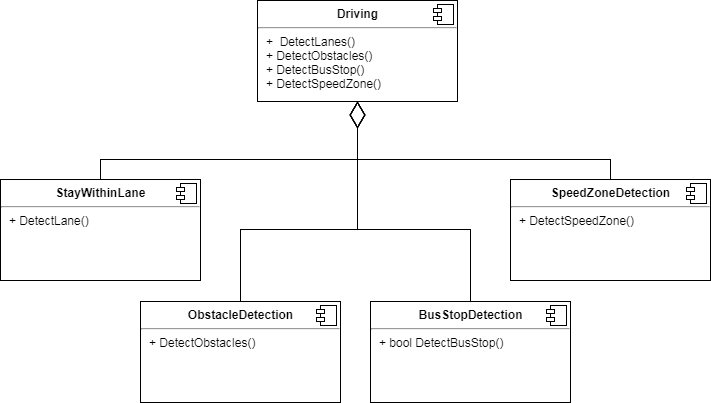
\includegraphics[width=\textwidth]{Images/Design/componentDiagram.png}
    \caption{Major components of functionality in the product; each component deals only with its own concerns}
    \label{fig:components}
\end{figure}

We split the program into five components, four of which contain one piece of functionality each. The last, the \code{Driving}-component is responsible for coupling the other components and for steering the bus based on their provided results. 

Note that while these components refer mostly to the software for the NXT, we cannot design the components in a vacuum. Specifically, incorrect sensor measurements, track/lane inconsistencies and similar situations need to be taken into account during programming, because otherwise, the product might not work as expected. 

In the following sections, we will consider this general architecture with a higher degree of granularity, to decide exactly how the software will work and how it will interact with the hardware. 


\subsection{Assumptions and Guarantees}
For now, we are imagining each component as a black box. What it contains is not of importance, only what it can do. Each component guarantees specific functionality as long as certain assumptions are met.

Most of the assumptions\todo{What assumptions in particular} are made for the sake of simplicity in order to not delude the design with unnecessary detail. In this section, we will specify assumptions and guarantees that are not immediately obvious. Other, common assumptions, however, like the fact that the bus needs gravity to drive properly, will still be left implicit. 

\begin{description}
    \item[Driving]
    We assume that the bus never spins its wheels without moving. We guarantee that the bus will drive the requested direction and distance. Because the track may be uneven, we cannot guarantee that the bus won't drive slower than the requested speed. 
    
    \item[ObstacleDetection]
    We assume that any obstacles are large and made out of material that can be detected consistently by the ultrasonic sensor. We guarantee that the bus will halt at any obstacles conforming to this style. 
    
    \item[StayWithinLane]
    The component assumes perfectly consistent road markings with no imperfections and unintentional holes. It also assumes that the bus was started at a valid point inside the road markings, where it still can physically manoeuvre the bus to stay within the lanes without reversing. It guarantees that the bus will not drive outside the road markings, at most with minor violations of a short duration (like any human driver might). 
    
    \item[SpeedZoneDetection]
    We assume that each different speed limit is marked with a single road marking that can be recognised and distinguished by a colour sensor. 
    
    %The component guarantees that it can park parallel to a bus stop with a maximum distance of 1 cm to the edge at any point. 
    % Rip this! :(

    \item[Stop Button]
    Although this fits less well with the reality, we will not be using a physical stop button inside the bus, because this will be tough to click. For this reason, the component assumes that it receives a Bluetooth signal, and will then ensure that the bus halts at the next stop.  
    
    \item[BusStopDetection]
    We assume that each bus stop is marked with a road marking that can be recognised by a colour sensor. The component guarantees that it will return true (which communicates that the bus should stop) when and only when there is this bus stop road marking below, and when it was told to stop by an external button.  
    
    
\end{description}